\documentclass{standalone}
\usepackage{tikz}
\usetikzlibrary{positioning,matrix,backgrounds}
\begin{document}

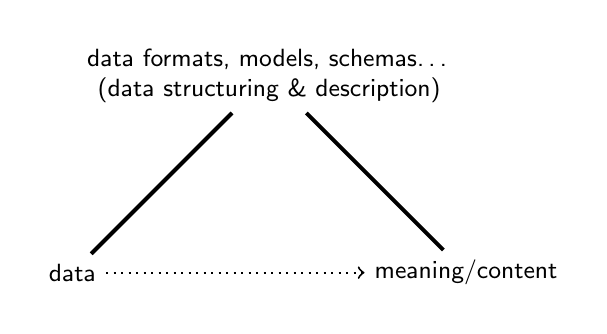
\begin{tikzpicture}[
    font=\sffamily\small,line width=0.25mm,
    show background rectangle,background rectangle/.style={fill=white}
]

\node (data) at (-25mm,0) {data};
\node (meaning) at (+25mm,0) {meaning/content};
\node[text width=50mm,align=center] (methods) at (0,25mm) 
    {data formats, models, schemas\ldots\\(data structuring \& description)};

\draw[dotted,->] (data.east) to (meaning.west);
\draw[line width=0.5mm] (data) to (methods) to (meaning);

\end{tikzpicture}
\end{document}
